\section{Model Exercise 2-2 (03): Pressure driven percolation (healing)}
\label{sec:mex03}
%------------------------------------------------------------------------------
\Authors{Mathias Nest, Keita Yoshioka et al.}
%------------------------------------------------------------------------------
\subsection{Experimental set-up}
%------------------------------------------------------------------------------
One of the most important properties of barriers formed by salt or clay is their ability to close cracks and heal through creep. This means, that the materials can regenerate and regain their impermeability, after damage due to, e.g. excavation activities or  pressure driven percolation because of a temporary violation of the minimal stress criterion.

\begin{figure}[!ht]
\centering
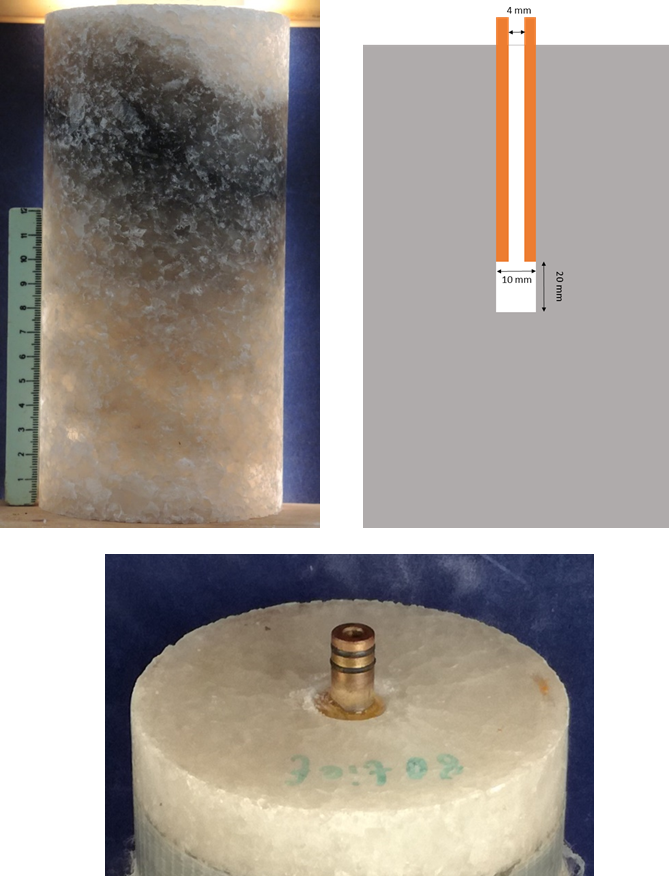
\includegraphics[width=8cm]{figures/mex3-exper-setup.png}
\caption{Rock salt sample, borehole geometry, detail of metal pipe.}
\label{fig:ME3-exper-setup}
\end{figure}

In this study we focus on the sealing of pathways and healing of cracks in salt and clay by measuring and simulating their gas permeability after damage has been done. To do so, we prepared cylindrical samples with a height of 20 cm and a diameter of 10 cm, with a borehole to the center, so that a gas pressure could be applied to a small area at the center. Initially all samples were placed under isostatic stress of 50 MPa for one day, to consolidate them. For the actual experiments the isostatic stresses were then changed to 10 MPa, 30 MPa, and 50 MPa, respectively. Before the gas pressure was applied, the plates which applied the axial stress were lock in place (''displacement boundary condition''). The gas pressure was increased in small steps, until a gas flow was detected. In all three cases a gas flow was detected before the percolation threshold was reached, which indicates that the samples suffered micro-fractures during preparation. After the last increase of the pressure, the flow rate was monitored for 24 to 70 hours under constant conditions.

\begin{figure}[!ht]
\centering
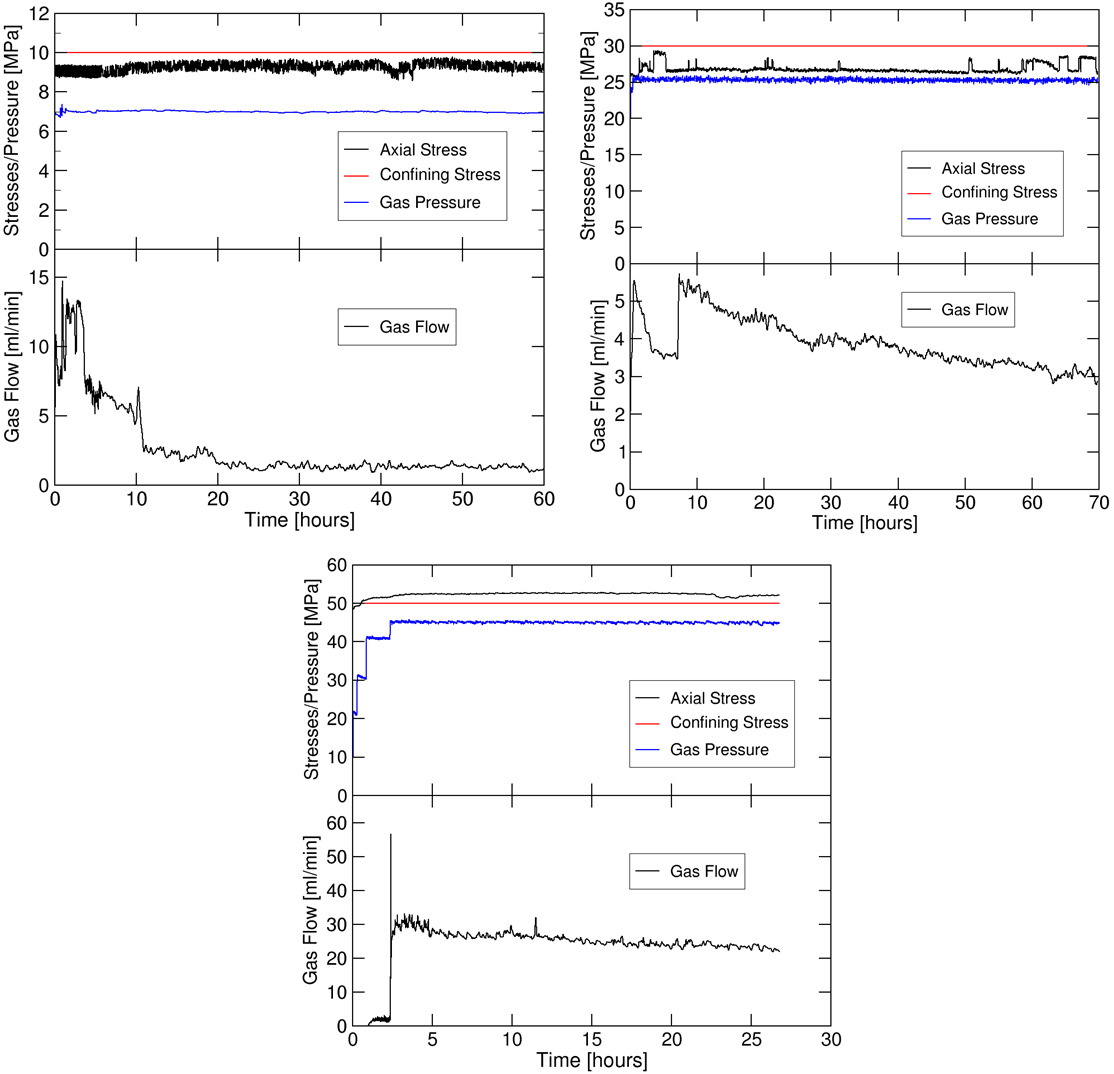
\includegraphics[width=1\textwidth]{figures/mex3-stresses-flows-v2.png}
\caption{Axial and confining stresses, gas pressures, and observed flow rates.}
\label{fig:ME3-stresses-flows}
\end{figure}
 
\begin{figure}[!ht]
\centering
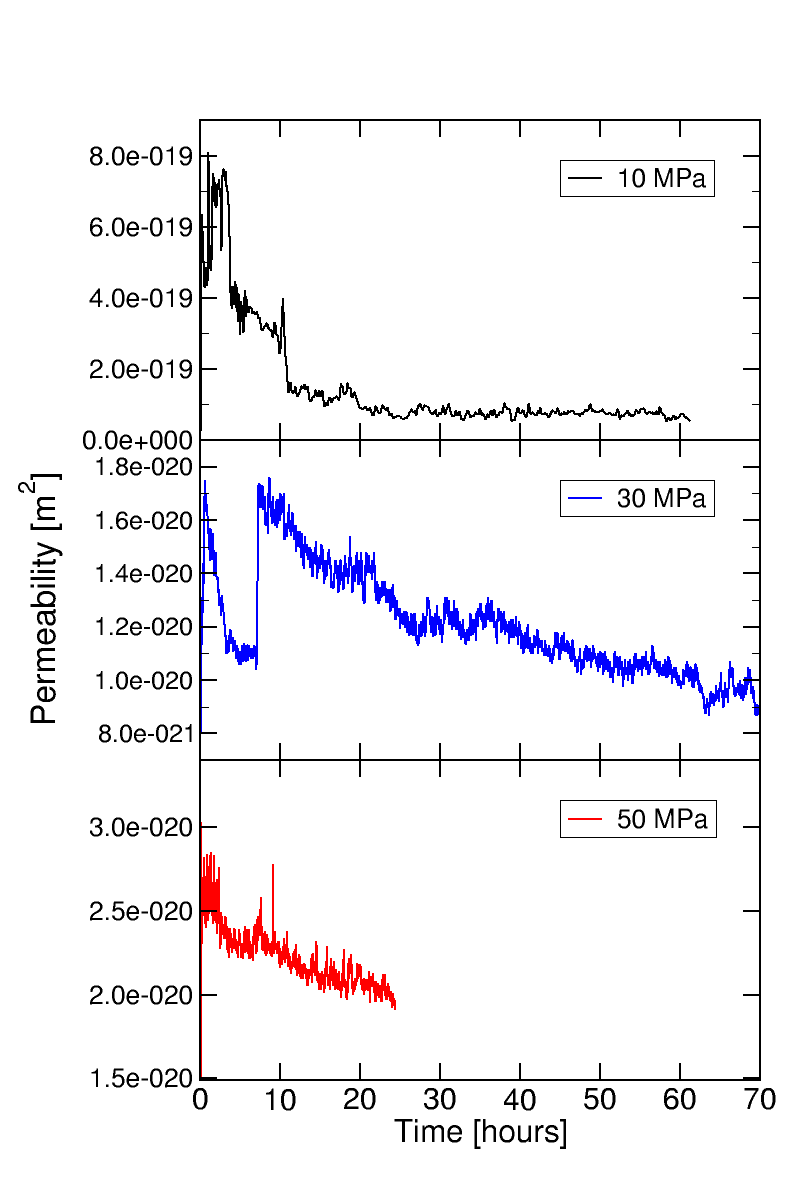
\includegraphics[width=9cm]{figures/mex3-perme-time-comparison.png}
\caption{Reduction of the permeability under different hydrostatic stress conditions.}
\label{fig:ME3-perme-exp}
\end{figure}

The flow rate can be converted into permeabilities, which are shown in Fig. \ref{fig:ME3-perme-exp}. For all three cases a reduction of the permeability is found,  showing that the cracks are narrowing and slowly closing. 
%------------------------------------------------------------------------------
\subsection{Model approaches}
%------------------------------------------------------------------------------
\subsubsection*{Discrete-Element-Model (DEM)}

\begin{figure}[!ht]
\centering
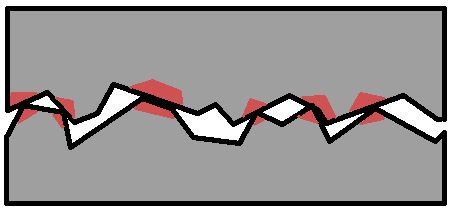
\includegraphics[width=9cm]{figures/mex3-crack-stresses.png}
\caption{Locations of high deviatoric stress in a crack. The deviatoric stress drives creep, which leads to a closing of the crack.}
\label{fig:ME3-crack-stre}
\end{figure}

\todo[inline]{[IfG]: Please add DEM simulation results}

\subsubsection*{Finite-Element-Model: Variational Phase-Field (VPF)}

\begin{figure}[!ht]
\begin{subfigure}[c]{0.49\textwidth}
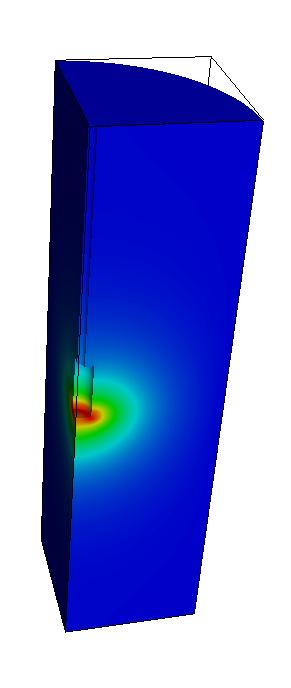
\includegraphics[width=1\textwidth]{figures/ME3_pres.png}
\subcaption{ME3 VPF model set up for the model exercise 3}
\label{fig:ME3_VPF_model}
\end{subfigure}
\hfill
\begin{subfigure}[c]{0.49\textwidth}
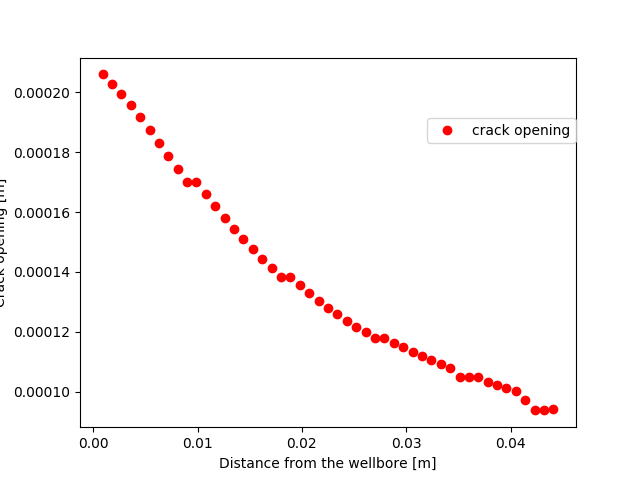
\includegraphics[width=1\textwidth]{figures/ME3_CrackWidth.png}
\subcaption{ME3 VPF crack width}
\label{fig:ME3_VPF_crack widht}
\end{subfigure}
\caption{ME3 VPF preliminary}
\end{figure}

\todo[inline]{[UFZ](KY): Please describe VPF simulation results}

%------------------------------------------------------------------------------
\subsection{Results and discussion}
%------------------------------------------------------------------------------
